\documentclass[../custom]{flashcards}
\usepackage{array}
\usepackage{enumitem}
\usepackage{booktabs}
\usepackage{multirow}
\usepackage{amsmath}
\usepackage{tikz}

\def\labelitemii{$\circ$}
\def\labelitemiii{$\diamond$}
\def\labelitemiv{$\cdot$}

\begin{document}
\cardfrontstyle{headings}

\cardfrontfoot{Study Session 4}
\newcommand{\studyArea}{Private Wealth Management}

\begin{flashcard}[\studyArea]{Tax Considerations for Mean Variance Optimization}
    \begin{flushleft}
        Ideally, the efficient frontier should be viewed on an after-tax basis. Because the tax status of an investment depends on the account it's in, it could appear on the efficient frontier in both taxable and non-taxable forms.\newline

        The mean-variance optimization should optimally allocate assets and determine the optimal asset location for each asset. Accrual equivalent after-tax returns would be substituted for before-tax returns, and risk on an after-tax basis would be substituted for before-tax risk.
    \end{flushleft}
\end{flashcard}

\cardfrontfoot{Study Session 13}
\renewcommand{\studyArea}{Alternative Investments}

\begin{flashcard}[\studyArea]{Advantages and Disadvantages to Direct Real Estate Investment}
    \begin{itemize}
        \item Advantages
        \begin{itemize}
            \item Many expenses are tax deductible.
            \item Ability to use more leverage than usual.
            \item Direct control of properties.
            \item Ability to diversify geographically.
            \item Lower volatility of returns than stocks.
        \end{itemize}
        \item Disadvantages
        \begin{itemize}
            \item Lack of divisibility.
            \item High information cost.
            \item High commissions.
            \item High operating and maintenance costs and management requirements.
            \item Geographic risks, such as neighborhood deterioration.
            \item Political risks, such as changing tax codes.
        \end{itemize}
    \end{itemize}
\end{flashcard}

\cardfrontfoot{Study Session 15}
\renewcommand{\studyArea}{Risk Management Applications of Derivatives}

\begin{flashcard}[\studyArea]{Box Spread}
    \begin{flushleft}
        Combination of a bull call spread and a bear put spread. That is, a long call and short put at $X_L$ and a long put and a short call at $X_H$. The payoff is always the same, regardless of the underlying price, which means assuming the prices are correct, the payoff is the risk-free rate.
        \begin{center}
            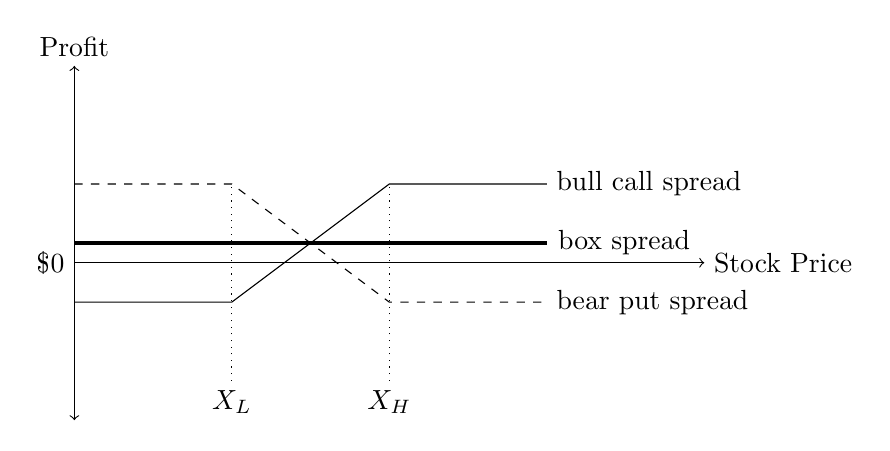
\begin{tikzpicture}
                \draw[<->] (0, -2) -- (0, 2.5) node[above] {Profit};
                \draw[->] (0, 0) node[left] {\$0} -- (8, 0) node[right] {Stock Price};
                \draw[dashed] (0, 1) -- (2, 1) -- (4, -0.5) -- (6, -0.5) node[above, right] {bear put spread};
                \draw (0, -0.5) -- (2, -0.5) -- (4, 1) -- (6, 1) node[above, right] {bull call spread};
                \draw[ultra thick] (0, 0.25) -- (6, 0.25) node[below, right] {box spread};
                \draw[dotted] (2, -1.5) node[below] {$X_L$} -- (2, 1);
                \draw[dotted] (4, -1.5) node[below] {$X_H$} -- (4, 1);
            \end{tikzpicture}
        \end{center}
    \end{flushleft}
\end{flashcard}

\cardfrontfoot{Study Session 16}
\renewcommand{\studyArea}{Trading, Monitoring and Rebalancing}

\begin{flashcard}[\studyArea]{Constant Proportion Portfolio Insurance}
    \begin{flushleft}
        Using CPPI, target weight varies with portfolio value and a specified minimum value. The difference is called the cushion. To get target allocation use
        \[
            \text{target investment} = M \times (\text{portfolio value} - \text{floor value}) = M \times (\text{cushion})
        \]
        where $M$ is the constant proportion for an asset class. To use CPPI, $M$ must be greater than $1$ and it doesn't change once selected.
    \end{flushleft}
\end{flashcard}

\cardfrontfoot{Study Session 17}
\renewcommand{\studyArea}{Evaluating Portfolio Performance}

\begin{flashcard}[\studyArea]{Diagram of Risk-Adjusted Measures}
    \begin{flushleft}
        \begin{center}
            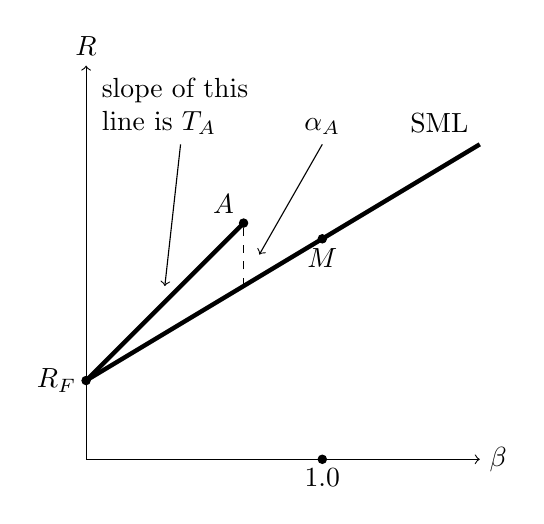
\begin{tikzpicture}
                \draw[->] (0, 0) -- (0, 5) node[above] {$R$};
                \draw[->] (0, 0) -- (5, 0) node[right] {$\beta$};
                \draw[ultra thick] (0, 1) -- (5, 4) node[above left] {SML};
                \draw[ultra thick] (0, 1) -- (2, 3);
                \draw[dashed] (2, 2.2) -- (2, 3);
                \draw[->] (3, 4) node[above] {$\alpha_A$} -- (2.2, 2.6);
                \draw[->] (1.2, 4) node[above, text width=2cm] {slope of this line is $T_A$} -- (1, 2.2);
                \draw[fill] (0, 1) circle[radius=1.5pt] node[left] {$R_F$};
                \draw[fill] (2, 3) circle[radius=1.5pt] node[above left] {$A$};
                \draw[fill] (3, 2.8) circle[radius=1.5pt] node[below] {$M$};
                \draw[fill] (3, 0) circle[radius=1.5pt] node[below] {1.0};
            \end{tikzpicture}
            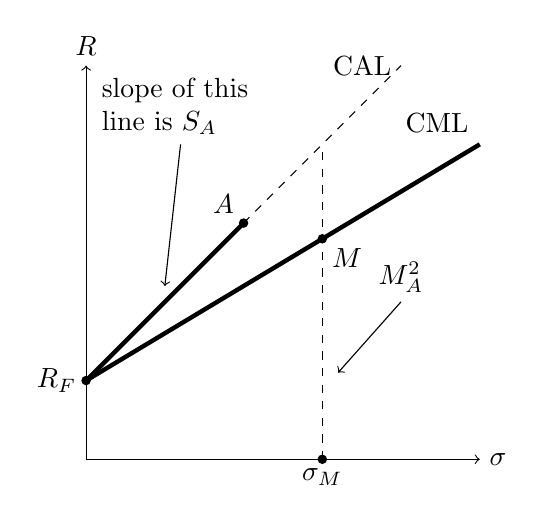
\begin{tikzpicture}
                \draw[->] (0, 0) -- (0, 5) node[above] {$R$};
                \draw[->] (0, 0) -- (5, 0) node[right] {$\sigma$};
                \draw[ultra thick] (0, 1) -- (5, 4) node[above left] {CML};
                \draw[ultra thick] (0, 1) -- (2, 3);
                \draw[dashed] (2, 3) -- (4, 5) node[left] {CAL};
                \draw[dashed] (3, 0) -- (3, 4);
                \draw[->] (4, 2) node[above] {$M^2_A$} -- (3.2, 1.1);
                \draw[->] (1.2, 4) node[above, text width=2cm] {slope of this line is $S_A$} -- (1, 2.2);
                \draw[fill] (0, 1) circle[radius=1.5pt] node[left] {$R_F$};
                \draw[fill] (2, 3) circle[radius=1.5pt] node[above left] {$A$};
                \draw[fill] (3, 2.8) circle[radius=1.5pt] node[below right] {$M$};
                \draw[fill] (3, 0) circle[radius=1.5pt] node[below] {$\sigma_M$};
            \end{tikzpicture}
        \end{center}
    \end{flushleft}
\end{flashcard}

\cardfrontfoot{Study Session 18}
\renewcommand{\studyArea}{Global Investment Performance Standards}

\begin{flashcard}[\studyArea]{GIPS Characteristics}
    \begin{itemize}
        \item Voluntary, minimum standards for performance presentation.
        \item Contain requirements and best practices.
        \item Only investment management firms can claim compliance.
        \item Provide a standard where local laws may not exist.
        \item Includes all actual, fee-paying, discretionary accounts in composites.
        \item Must present five years of history, or since inception.
        \item Must use prescribed calculations and provide disclosures.
        \item Goal of full disclosure and fair representation.
        \item In cases of conflict, the local law should be followed.
        \item Encourages monitoring processes and controls.
        \item Must document the polices used.
    \end{itemize}
\end{flashcard}
\end{document}
